\documentclass[tikz,border=1pt]{standalone}
% Drawn at its printed size (17.7 cm, inside the 18.2 cm IEEE \textwidth): include it unscaled so that
% box text stays 8 pt and notes 7 pt, matching the matplotlib figures. Times matches the IEEEtran body.
\usepackage[T1]{fontenc}
\usepackage{newtxtext,newtxmath}
\usetikzlibrary{arrows.meta,positioning}
\definecolor{ink}{HTML}{222222}
\definecolor{muted}{HTML}{5F6B73}
\definecolor{bluefill}{HTML}{E3EDF7}
\definecolor{blueedge}{HTML}{1F5A96}
\definecolor{tealfill}{HTML}{E0F1EE}
\definecolor{tealedge}{HTML}{137A72}
\definecolor{orangefill}{HTML}{FBEBD9}
\definecolor{orangeedge}{HTML}{C0611A}
\definecolor{purplefill}{HTML}{ECE5F4}
\definecolor{purpleedge}{HTML}{6C4C93}
\definecolor{grayfill}{HTML}{F3F4F5}
\definecolor{grayedge}{HTML}{68757D}
\tikzset{
  >={Latex[length=1.8mm,width=1.2mm]},
  every node/.style={text=ink, font=\fontsize{8}{9.5}\selectfont, inner sep=0pt},
  panel/.style={draw, rounded corners=2pt, line width=.5pt, minimum height=4.3cm, anchor=south west},
  item/.style={draw, rounded corners=1.5pt, line width=.45pt, fill=white, minimum height=.5cm, inner xsep=3pt, align=center},
  title/.style={font=\bfseries\fontsize{8}{9.5}\selectfont},
  note/.style={font=\fontsize{7}{8.4}\selectfont, text=muted, align=center},
  flow/.style={->, line width=.6pt, draw=ink},
}
\begin{document}
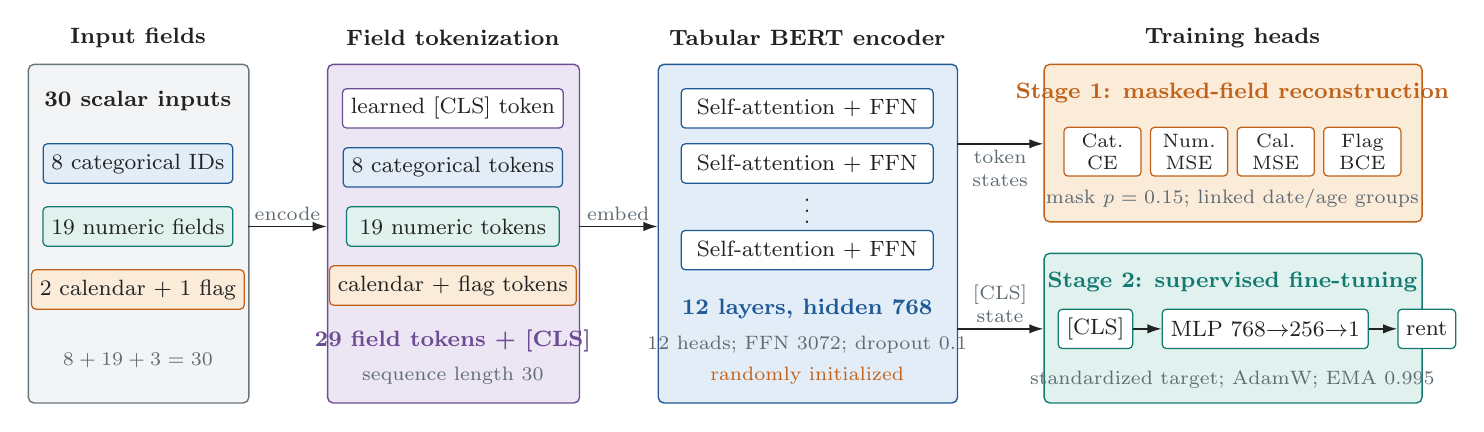
\begin{tikzpicture}[x=1cm,y=1cm]
  % Four equal-height columns; x extents: 0-2.8, 3.8-7.0, 8.0-11.8, 12.9-17.7.
  \foreach \x/\t in {1.4/Input fields, 5.4/Field tokenization, 9.9/Tabular BERT encoder, 15.3/Training heads}
    \node[title] at (\x,4.65) {\t};

  % Inputs.
  \node[panel, fill=grayfill, draw=grayedge, minimum width=2.8cm] (in) at (0,0) {};
  \node[title] at (1.4,3.85) {30 scalar inputs};
  \node[item, draw=blueedge, fill=bluefill, minimum width=2.4cm] at (1.4,3.05) {8 categorical IDs};
  \node[item, draw=tealedge, fill=tealfill, minimum width=2.4cm] at (1.4,2.25) {19 numeric fields};
  \node[item, draw=orangeedge, fill=orangefill, minimum width=2.4cm] at (1.4,1.45) {2 calendar + 1 flag};
  \node[note] at (1.4,.55) {$8+19+3=30$};

  % Tokens.
  \node[panel, fill=purplefill, draw=purpleedge, minimum width=3.2cm] (tok) at (3.8,0) {};
  \node[item, draw=purpleedge, minimum width=2.7cm] at (5.4,3.75) {learned [CLS] token};
  \node[item, draw=blueedge, fill=bluefill, minimum width=2.7cm] at (5.4,3.0) {8 categorical tokens};
  \node[item, draw=tealedge, fill=tealfill, minimum width=2.7cm] at (5.4,2.25) {19 numeric tokens};
  \node[item, draw=orangeedge, fill=orangefill, minimum width=2.7cm] at (5.4,1.5) {calendar + flag tokens};
  \node[title, text=purpleedge] at (5.4,.8) {29 field tokens + [CLS]};
  \node[note] at (5.4,.35) {sequence length 30};

  % Encoder.
  \node[panel, fill=bluefill, draw=blueedge, minimum width=3.8cm] (enc) at (8.0,0) {};
  \node[item, draw=blueedge, minimum width=3.2cm] at (9.9,3.75) {Self-attention + FFN};
  \node[item, draw=blueedge, minimum width=3.2cm] at (9.9,3.05) {Self-attention + FFN};
  \node at (9.9,2.55) {$\vdots$};
  \node[item, draw=blueedge, minimum width=3.2cm] at (9.9,1.95) {Self-attention + FFN};
  \node[title, text=blueedge] at (9.9,1.2) {12 layers, hidden 768};
  \node[note] at (9.9,.75) {12 heads; FFN 3072; dropout 0.1};
  \node[note, text=orangeedge] at (9.9,.35) {randomly initialized};

  % Stage 1 head.
  \node[panel, fill=orangefill, draw=orangeedge, minimum width=4.8cm, minimum height=2.0cm] (s1) at (12.9,2.3) {};
  \node[title, text=orangeedge] at (15.3,3.95) {Stage 1: masked-field reconstruction};
  \foreach \x/\t in {13.65/Cat.\\CE, 14.75/Num.\\MSE, 15.85/Cal.\\MSE, 16.95/Flag\\BCE}
    \node[item, draw=orangeedge, minimum width=.98cm, minimum height=.62cm, font=\fontsize{7}{8}\selectfont] at (\x,3.2) {\t};
  \node[note] at (15.3,2.6) {mask $p=0.15$; linked date/age groups};

  % Stage 2 head.
  \node[panel, fill=tealfill, draw=tealedge, minimum width=4.8cm, minimum height=1.9cm] (s2) at (12.9,0) {};
  \node[title, text=tealedge] at (15.3,1.55) {Stage 2: supervised fine-tuning};
  \node[item, draw=tealedge, anchor=west] (cls) at (13.08,.95) {[CLS]};
  \node[item, draw=tealedge, right=.36cm of cls] (mlp) {MLP $768{\to}256{\to}1$};
  \node[item, draw=tealedge, right=.36cm of mlp] (rent) {rent};
  \draw[flow] (cls) -- (mlp);
  \draw[flow] (mlp) -- (rent);
  \node[note] at (15.3,.3) {standardized target; AdamW; EMA 0.995};

  % Data flow between columns; labels sit above the arrows inside the 1.0-1.1 cm gaps.
  \draw[flow] (2.8,2.25) -- node[note, above=2pt] {encode} (3.8,2.25);
  \draw[flow] (7.0,2.25) -- node[note, above=2pt] {embed} (8.0,2.25);
  \draw[flow] (11.8,3.3) -- node[note, below=2pt] {token\\states} (12.9,3.3);
  \draw[flow] (11.8,.95) -- node[note, above=2pt] {[CLS]\\state} (12.9,.95);
\end{tikzpicture}
\end{document}
